\chapter{Design and Implementation}\label{C:work}

A large portion of the project was gaining enough understanding of the existing work on RBMs to be able to implement the ORBMs algorithm and architecture. This was crucial as bugs in the implementation are a threat to validity.

\todowording{Make sure you talk about why the sigmoid is the most appropriate atrication function! Maybe this should go in background..}

%A large amount of the accomplishments in the project so far have been in gaining the understanding needed to really explore and verify this new technique - given it is built upon the existing work of Restricted Boltzmann Machines. This understanding means that robust correctness tests can be written. This in turn ensures that results produced have more credibility, so the implementation is known to be sound. %

\section{Evaluation Dataset Choice}

\begin{itemize}
  \item 2 Bit XOR - It's the minimal case. Can examine reconstructions and dreams/fantansy emperically. Also can check that code performs as expect by manually calcating expected values for the algorithm.
  \item X Neighbouring Bits On in Y Bit Pattern - A natural next step from 2 bit XOR. Still trivial to train an RBM to represent, quick feedback to ensure the algorithm works. Allows comparing the different approximations tractable as number of hidden units is small enough.
  \item Square Patterns in a 5 by 5 Pixel Image - Another natural step from neighbouring bits, trival to construct a dataset. Very easy to compose. Can use the same model for both models in the ORBM Architecture.
  \item Rectangles in a 5 by 5 Pixel Image - Next step, builds on the previous test but adds a different model for each source. Also different shapes of model can be used.
  \item Continous Rectangles (Pixel values 0 to 1) in a 5 by 5 Image - Another variation working towards the MNIST dataset, same as the previous but has continous visible pixels. Allows to different intensitities, interesting cases where the images overlap and increase in intensity.
  \item MNIST Handwritten Digit Dataset - Pixel values from 0 to 1, 28 by 28 pixel image (784 pixel features.) Used extensiviely in previous studies. Gives me confidence that RBMs can learn these representations. Also allows metaparameters don't have to be tweaked as much as studies already have found reasonable values. Non-trivial to evaluate, but more of a real world case.
\end{itemize}

\section{Implementation Design}

\subsection{Language Choice}
\begin{itemize}
  \item Library choice meant efficiency with benefits of python for quick dev
  \item Easy to deploy to grid (versus java higher risk, lack of expeirence)
  \item Ordering of evaluation tasks made unit testing, with hand made test cases possible. Also less risk, remove the uncertainty around the RBM.
  \item testing approach
\end{itemize}


\subsection{Program Architecture}

The program was implemented with unit testing and composability in mind. It was important that the design supported comparing the Full and Approximated correction. By using Python, multiple inheritance could be leveraged. For instance  adding continuous pixel value support to the \texttt{Full Correction Sampler}, one simply needed to extend \texttt{Continuous Approximate Correction Sampler} and the  \texttt{Full Correction Sampler}, with no code actually in the new class. The architecture is pictured in the class diagram \ref{F:Prog-Arch}. There were three main roles these classes filled:
\begin{enumerate}
  \item The \texttt{Trainer} was used to train the weights of a supplied \texttt{RBM}. It would do so using a supplied \texttt{sampler}, decoupling how samples were generated from the training process.
  \item The \texttt{RBM} was the model of an RBM, storing the weight matrix, as well as parameter information. Also this supported conversion of the SciPy Sklearn libraries' RBM implementation into the implementation used in this project. Decoupling the concept of an \texttt{RBM} from the \texttt{Sampler} and the \texttt{Trainer} meant that RBMs could be `plugged` into the ORBM architecture with ease.
  \item The \texttt{Sampler} defined how to perform Gibbs sampling, the subclasses defining whether it is standard RBM sampling or ORBM sampling. This made is trivial to compose samplers, which was required for the ORBM samplers.
\end{enumerate}

\begin{figure}[h]
\begin{center}
  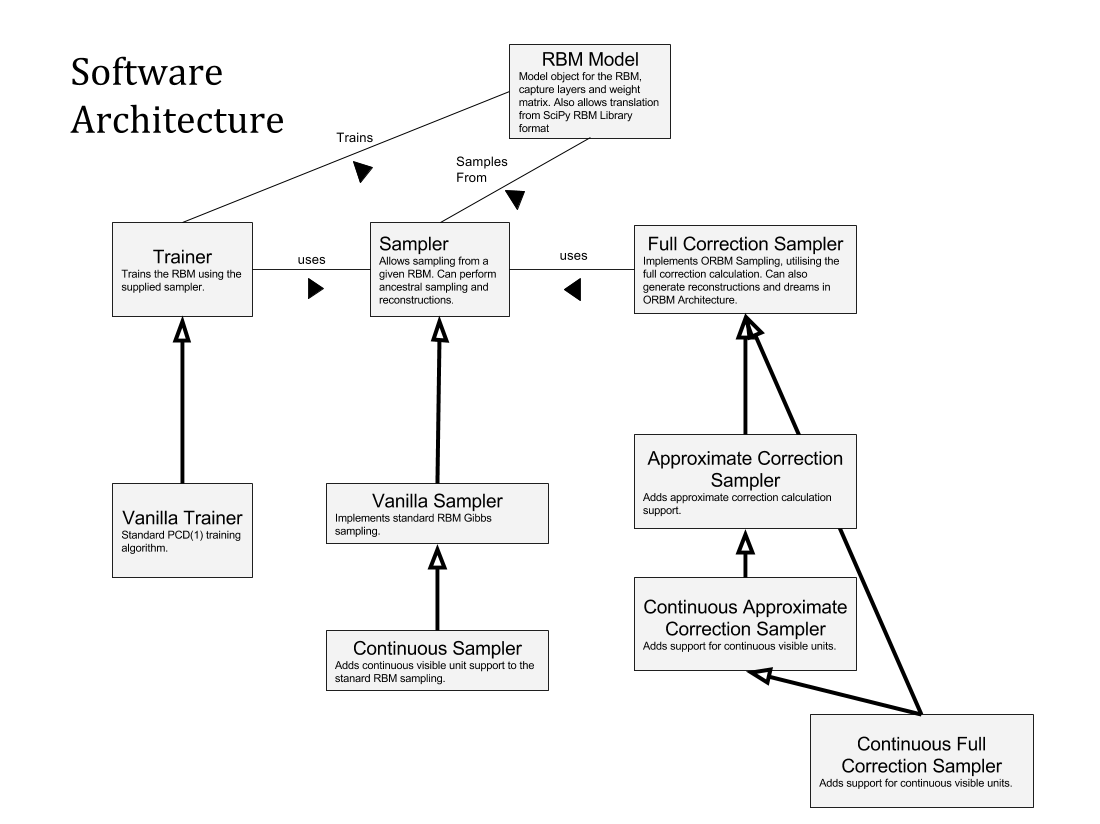
\includegraphics[width = 0.8\textwidth]{Assets/ENGR489-Architecture.png}
\caption{A figure showing the architecture for the implemented test suite in UML notation.}
\label{F:Prog-Arch}
\end{center}
\end{figure}

% \subsection{Language Choice}\label{SS:language}
%
% The project is currently implemented using Python 3.4, however three other languages were considered for this project, Matlab, R and Java.
% Several factors were considered that lead to this decision.
%
% \begin{description}
% \item[Efficiency]A large amount of data is required to train a Restricted Boltzmann Machine and the new approach has a higher complexity than the traditional RBM implementation. The language choice should not prevent the algorithm from being run in reasonable time, as this would hamper the ability to test it for correctness and performance.
% \item [Ease of use]The project requires significant up front learning which means some familiarity with the language or a shallow learning curve will help keep velocity/progress high. The focus can then be on understanding the required theory instead of language niches.
% \item  [Support for testing]From a correctness standpoint, being able to evaluate the algorithms will require confidence of a correct implementation and therefore help lend credibility to subsequent findings.
% \item [Machine Learning Library support]Being able to leverage libraries allows the focus to be on implementing and testing the new algorithm.
% \item [Stakeholder collaboration]The projects supervisor who conceived the new approach inherently has a good understanding of how it works and therefore having a language they are comfortable working in can help with ensuring implementation correctness. For instance pair programming has been employed which is facilitated by a programming language common to both developers.
% \end{description}
%
% All of the languages considered have the efficiency for machine learning tasks, despite Python being on the slower end of the spectrum of languages, versus that of the compiled JVM languages like Matlab or Java, it is still fast enough. The complexity of the traditional RBM is relative to what is trying to be modelled, less of the language implementing it.
% Java and Python have robust testing suites given they are used for non-academic goals. Matlab and R do have suites however the author has not had experience with them. Choosing from one of these two languages would increase the amount of upfront learning required and therefore increase this risk.
% The author had the most experience with Python and Java, however Python was favoured due to it's Matlab-like library NumPy. Expressive matrix syntax combined with the familiarity and brevity of Python made it a compelling option.
%
% \subsection{Library Choice}\label{SS:Lib}
%
% Considerations regarding library choice only really apply to the part of the system that needs to be robust, the number crunching.
%
% Given the choice of Python, the decision to use the NumPy library was almost inherent. NumPy is a linear algebra library that offers fast implementations of matrix operations in a concise, expressive syntax. For instance, a whole training set of images, each image of size $ x^2 $, represented by a $ 3 $ by $ x$ by $x $ matrix, can then be operated on all at once. Also NumPy is interoperable with open source Python Machine Learning Libraries. For instance Scikit-Learn \cite{scikit-learn} and Theano \cite{bergstra+al:2010-scipy} which allows greater reproducibility in my results. Finally, it is a mature, well tested library, being an evolution of the Numeric python library which started developing in 1995 \cite{2015HistSciPy}.
% %
% \subsection{Dataset Choice}
%
% A crucial part of the project is ensuring that the tests can be reproducible, allowing any results to be used as evidence in a paper. Hence the importance of choose a dataset that has some credibility or can allow this approach to be compared to existing work. The MNIST digit dataset was originally chosen as a good dataset for this projects tests. There has been work using RBMs \cite{Hinton:2006dk} and other machine learning approaches \cite{Lecun:1998hy},  to represent these handwritten digits previously. This gives a point of reference to compare performance.
%
% It is worth noting: In section \ref{SS:HDR} it is highlighted that the results from testing with this dataset are not outstanding, hence a more minimal toy-dataset is being used until more understanding can be gained about what is and is not working.
%
% \section{Implementation}\label{S:Implementation}
%
% The traditional Restricted Boltzmann Machine has been implemented.
%
% The new theory applies a correction when constructing the hidden representation of the noisy input. This correction allows each model (RBM) to take responsibility for different parts of the input data.
%
% The calculation of this correction introduces a dependency between the hidden units and therefore we sacrifice some efficiency for better performance on multi-cause data.
% The full, un-approximated correction calculation has been implemented and connected to the Restricted Boltzmann Machine.
%
% Tests have been created to verify if the new approach is working.
% As RBMs are generative models, we can show them an input and have them generate their own recreation based on the internal representation. This recreation is dependant on the image it was created from and therefore could be used for a performance test.
% We can approximate the likely-hood of, given a noisy image, how well can we reconstruct the underlying clean image. This forms a 'score' for the $ith$ pixel of an image.
%
% $$  P( v_i' | v_i^{composite}) = P(v_i' | v_i^{clean}  ) $$
%
% Where $ v_i' $ is the reconstruction based on the RBMs internal representation. $ v_i^{composite} $ is the composite (noisy) image and $ v_i^{clean} $ is the clean image; the underlying model that noise is added to to create the composite image.
%
% This score can then be approximated image-wise and compared to the traditional approach, by sampling (creating reconstructions). From this we can see which images the new approach performs better/worse.
%
% \subsection{Handwritten Digit Recognition}\label{SS:HDR}
%
% The performance tests described in section \ref{S:Implementation} have been implemented for all digits in the MNSIT Handwritten Digit dataset \cite{mnistlecun} and the results are not outstanding. A toy model of a horizontal bar acts as the noise and is composed with the digit dataset to create the noisy input. We see this in \ref{F:digit_example}. The Noisy Input is the composite image, this is what the reconstructions pictured in New Approach and Traditional Approach were generated from. The target was generated from the underlying (non-composited) '2' images.
%
% \begin{figure}[htbp]
% \begin{center}
% 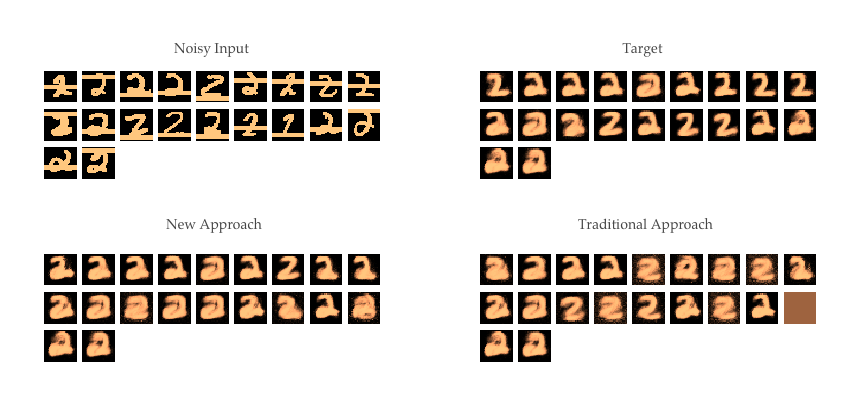
\includegraphics[width=1\textwidth]{Assets/Initial_Results}
% \caption[Initial results using new approach on noisy handwritten two images.]{Initial results using new approach on noisy handwritten two images. The input was 20 MNIST two digits with a random 4 pixel high bar composited. The new technique does not perform better by much over the dataset.  }
% \label{F:digit_example}
% \end{center}
% \end{figure}
%
%
% Another performance test carried out has been classification performance. The hypothesis being that the new approach should be able to generate a better representation despite having noisy training and test sets. The actual classification is deferred to an AI classifier that is trained on the hidden representations.
% Fig \ref{F:rbmClassification} shows a visual representation of this. The RBM is trained on some data, then a hidden representation and known labels are used to create a transformed training and test set which a perceptron or other classifier is then trained on. The better the classification performance the better representation the model has achieved.
% \begin{figure}[htbp]
% \begin{center}
% 	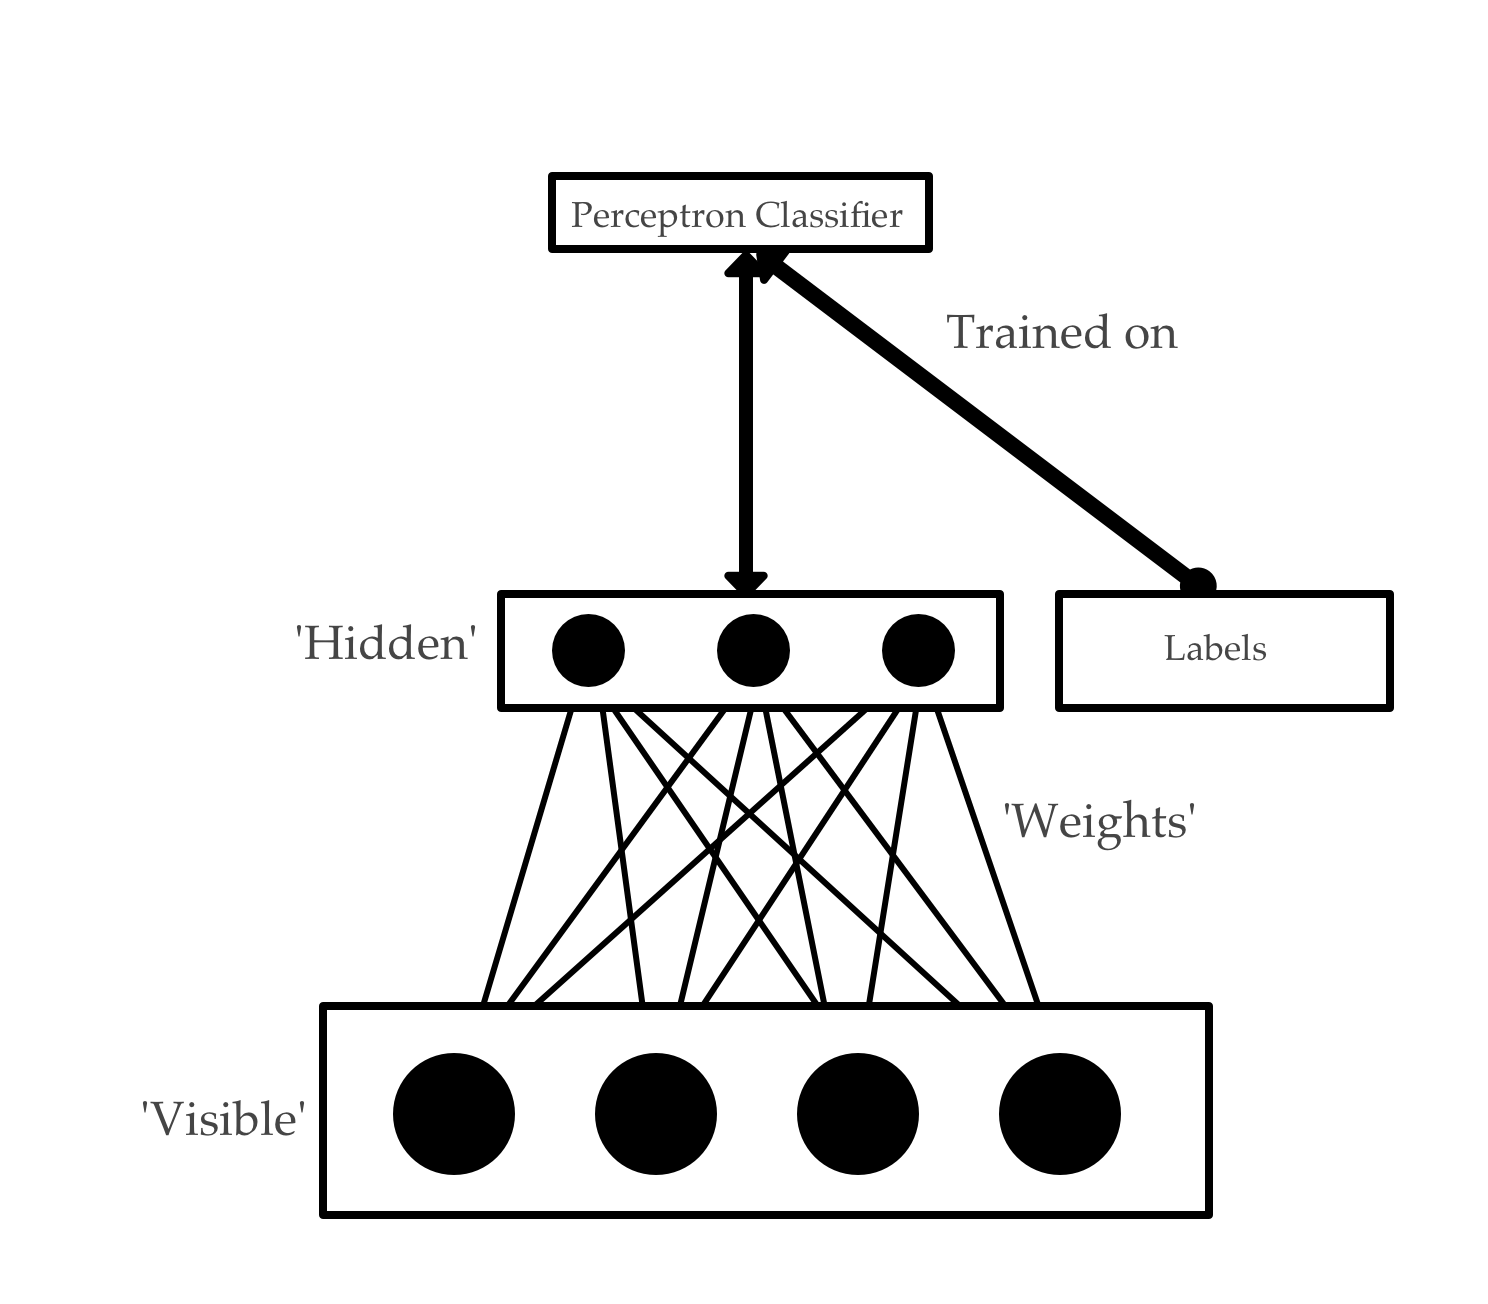
\includegraphics[width=0.7\textwidth]{Assets/RBMClassification}
% \caption[Figure demonstrating how classification can be applied using an RBM]{Figure demonstrating how classification can be applied using an RBM. }
% \label{F:rbmClassification}
% \end{center}
% \end{figure}
%
% \begin{figure}[htbp]
% \begin{center}
% 	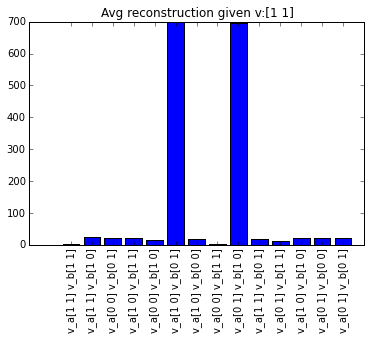
\includegraphics[width=0.7\textwidth]{Assets/yup}
% \caption{Figure showing the results of generating reconstructions using the new approach and two identical RBMs that can recognise a single pixel being on a time.}
% \label{F:twobit}
% \end{center}
% \end{figure}
%
% The non-outstanding results shown in \ref{F:digit_example} and the other digits, highlighted that some minimal test cases need to be satisfied before more complicated models like digits can be explored. The tests currently in place are not atomic enough.
%
% We arrived at the minimal test case, a two bit image, with binary pixels and a toy RBM model trained to understand one pixel being on at a time. This had the advantage of being able to be checked by hand and approximations of the correction could be explored in the minimal case. This is the  smallest case possible for them to actually work and as a result, more robust correction tests have been constructed.
%
% In the two bit scenario it is very easy to measure the performance of reconstructions, we would hope given an visible input of $ v = [1,1] $ that the new approach would most of the time result in reconstructions from the two models of $ v'_A = [1,0]$,  $v'_B = [0,1] $ and conversely $ v'_A = [0,1]$,  $v'_B = [1,0] $. Where $v'_A$ is the reconstruction generated, given $v$ from model A.
%
% The results of doing this in a two bit system, that is two hidden and two visible units resulted in the plot in fig \ref{F:twobit}. We see the most common reconstructions are those defined above. It is important to look at the reconstructions from both models holistically to ensure they are actually separating the sources. The figure shows the average of 1000 runs of the new approach, the two bit example making this many runs quite feasible with so few features.
%
%
% \section{Evaluation Planning}\label{S:evaluation}
%
% As the output of the project is essentially a series of reproducible performance results, it is important that the algorithm is sound in practice and matches what the theory describes. The validity of the results hinge on the confidence that the code does what it should. This precondition is enforced by unit and integration testing the system. The third party libraries in use for linear algebra (NumPy) and plotting (Matplotlib) are well tested and feature in other peer reviewed literature in the field of Machine Learning \cite{Millman:2011wp}.
%
% As touched on in the scope changes in section \ref{S:ScopeChanges} the evaluation phase of the project needs to be ongoing. The performance of the new approach needs to be checked at every point to ensure that cases where the new approach does and does not work can be pinpointed. It also makes tracking down what factors make it more or less effective easier.
% The actual approach to evaluation is touched on above, but it amounts to verifying if and when the new approach generates a better representation of a composite image versus that of the traditional approach.
